\chapter{Covariate modeling}
\label{theory-covariate_modeling}
As I have mentioned frequently in previous sections, the
epidemiological data on disease morbidity collected in systematic
review is often very sparse and very noisy.

Covariate modeling is a method to explain the variation in noisy
data in terms of demographic, epidemiological, and study-specific
variables.  This is often challenging because there is no particularly
explanatory variable available, and also because the data are very
sparse.  Nonetheless, this approach has a long history of relevant
application in global health.\cite{girosi_demographic_2008,jon_wakefield_bayesian_1996,TK_at_least_3_more_citations,TK_at_least_3_more_citations,TK_at_least_3_more_citations}

In the integrative systems model of disease in populations, covariate
modeling has two distinct goals.  One is to
explain the bias and variation of the noisy measurements of
epidemiological rates.  For example, covariates can be used as a mechanism
for data-driven ``cross-walks'' to convert between alternative diagnostic methods
that have different sensitivities, and can also be used to
objectively down-weight data that comes from a noisier source such as
from nonrepresentative subpopulations that are not systematically
biased above or below the mean.

The other goal in covariate modeling is to use covariates
to increase the accuracy of out-of-sample predictions.  This
is accomplished by modeling the relationships between the disease
parameters of interest and the explanatory covariates. The modeled
relationships are then used to extrapolate predictions for the disease
parameters to geographic regions where covariate data is available,
but no direct measurements have been made.

In covariate modeling, there is often a distinction made between
``fixed effects'' and ``random effects.''  Bayesian approaches, such
as hierarchical modeling, blur this distinction (to the point that
hierarchical modeling is somtimes called ``mixed effect'' modeling.
\cite{Gelman_Multilevel_2005}  To make the nomenclature more
complicated, different methodological traditions of covariate modeling
have opposite concepts of what is fixed and what is random in effects.

For integrative systems models of disease, I have used fixed and
random effects in different ways, which makes them easy to keep
separated.  While I have used fixed effects for covariates that vary
by study or by country-year, I have only used random effects to model
indicator covariates for geographic units.

Sometimes I have constrained the random effects to sum to zero at each
level of a geographic hierarchy, which is an extension of the
traditional meaning of random effects in linear regression, where the
population mean of a random effect is zero.  In other models, it is
sufficient to use a prior with mean zero for the random effects, as is
the common approach in Bayesian modeling.  In either case, my random
effects always have a hyper-parameter for the dispersion, which allows
the model to infer how dispersed the random effects are between
geographic regions, and hence quantify the uncertainty in the
geographic regions for which no data is available.

These concepts will all be elaborated on in turn in the following
sections of this chapter.

\section{Fixed effects to explain bias}

A prototypical example comes from myocardial infarction (MI)
incidence, where there are a variety of diagnostic tests available.
Different studies of MI incidence use different diagnostic criteria
for case ascertainment.  The newer class of tests, which are based on
measuring levels of the blood protein troponin, are more sensitive
than earlier methods, and this leads to variation in data with a clear
explanation.  Figure~\ref{cov-sim} shows simulated data with a
covariate that has an effect like a troponin-based test might, raising
the number of observed cases by 30\%. By including an indicator
variable as a covariate in each row of data, $x_i = 1$ if row $i$
comes from a study that used a troponin test, and $x_i = 0$ otherwise,
I can fit a model which includes a parameter to cross-walk between
studies using these two different case ascertainment criteria.

\begin{figure}[h]
\begin{center}
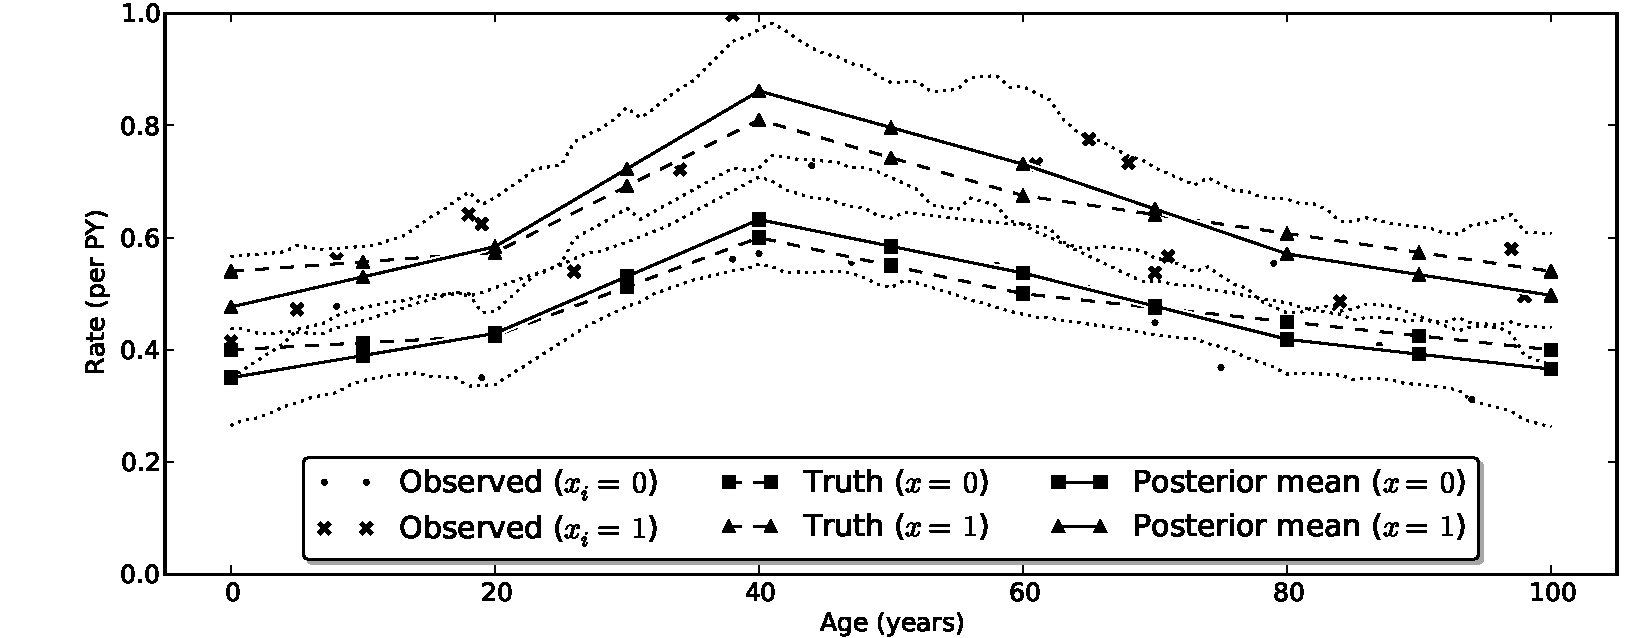
\includegraphics[width=\textwidth]{cov_fe.pdf}
\caption{Simulated dataset where different measurement techniques
  yield systematically different values. The data with $x_i=1$ are on
  average 30\% higher than data with $x_i=0$, and the covariate model
  recovers this difference accurately, with sufficient data.}
\label{cov-sim}
\end{center}
\end{figure}

This same approach can be applied to data on psychological disorders gathered with alternative recall periods, an application that arises frequently in the
meta-analysis of psychological disorders.  For example, in measuring
the population prevalence of bipolar disorder, many studies ask about
the existance of symptoms in the past month, while many others ask
about the past year.  Figure~\ref{bipolar-data-cv} shows the data
collected in systematic review for bipolar disorder, where past year
prevalence is higher than past month prevalence, because of the
episodic nature of the condition.

\begin{figure}[h]
\begin{center}
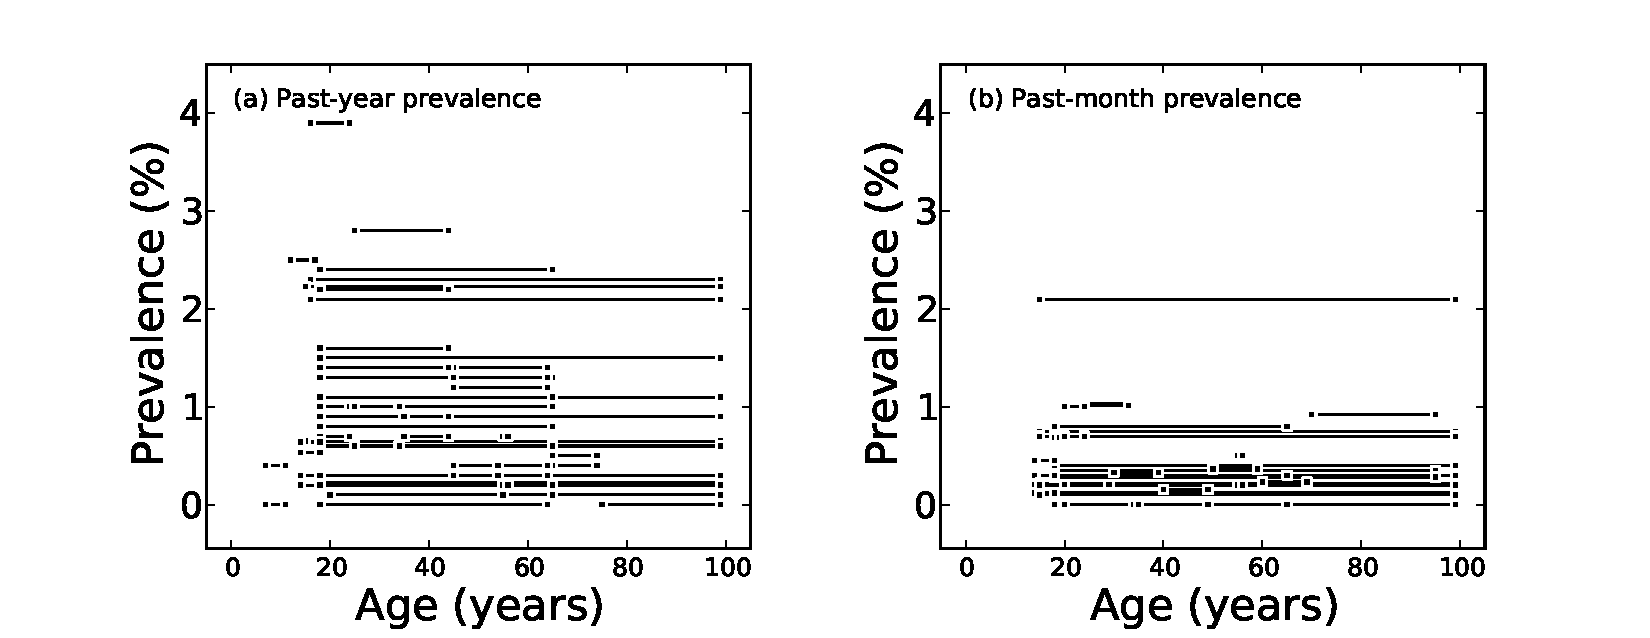
\includegraphics[width=\textwidth]{bipolar-data-by-cv.pdf}
\caption{Data on bipolar disorder collected in systematic review.
  Some studies measured past year prevalence, while others measured
  past month prevalence.  Because of the episodic nature of the
  condition, past month prevalence is $30$ to $40\%$ lower than past
  year prevalence.}
\label{bipolar-data-cv}
\end{center}
\end{figure}


In general, let the data collected in systematic review be denoted by
tuples $\left(a_i, n_i, r_i, X_i\right)$, where $a_i$ is the age
group, $n_i$ is the effective sample size, $r_i$ is the observed rate
value, and $X_i$ is a vector of covariate values. Then, using
$\scD(\pi, \rho; n_i)$ to denote the rate model, the fixed-effect
covariate model is then the following:
\begin{align*}
r_i &\sim \scD\left(\mu_i, \delta; n_i\right),\\
\mu_i &= h(a_i)e^{\beta X_i}
\end{align*}

The parameter $\beta$ represents the effect coefficients for
the fixed effects, and because the data are often sparse and noisy, it
can help the stability of the computational algorithms to put a weakly
informative prior on $\beta$, such as
\[
\beta_j \sim \Normal\left(0, 1^2\right) \text{ for } j = 1, \ldots, J.
\]
Of course, if experts have beliefs about the sign or magnitude of the
effect coefficient, this can be included as a more informative prior.

Two subtle choices are worth additional investigation in fixed effect
modeling: reference values and normalization.  Both of these choices
are known to influence the performance of computational
algorithms.\cite{gelman_bayesian_2003} For example, nonnormalized covariates can produce
nonconvergence in hill-climbing algorithms that work fine with
normalized covariates.  But because of the Bayesian priors and
especially because of the consistency from the compartmental model,
the choices are particularly important in this setting.

The term \emph{reference value} is borrowed from fixed effects
modeling of categorical variables, where so-called dummy variables
(zero/one indicators) are introduced for all but one category. When
all the dummy covariates are set to zero, the model produces
predictions for the reference category. In the formulation above, the
analogous notion occurs when $X_i = (0, 0, \ldots, 0)$.  Then the
expression for $\mu_i$ simplifies to
\[
\mu_i = h(a_i) e^{\beta \0} = h(a_i).
\]
It is this $h$ that is used as the age-specific rate function in
the compartmental model (as developed in
Chapter~\ref{theory-system_dynamics}), so the consistency between
incidence, prevalence, remission, and mortality is enforced at the
reference values.

Because the reference values are consistent, they must be chosen with
care.  For example, in the case of MI above, where some studies used
troponin based diagnostics and some did not, the reference value
should be \emph{with} troponin tests, because this is considered to be
more accurate.

A concrete example using the bipolar disorder data can make this
clearer.  Chapter~\ref{bipolar} develops the consistent model for
bipolar disorder in detail, which is used here in two variations.
First, when the past year prevalence is used as the reference
value, and second when the past month prevalence is used as the
reference.  This changes the predicted prevalence, of course, but it
also changes the predicted incidence (for which little data is
available).  Figure~\ref{bipolar-ref-alts} shows how the alternative
reference values change the incidence estimate in this case.


\begin{figure}[h]
\begin{center}
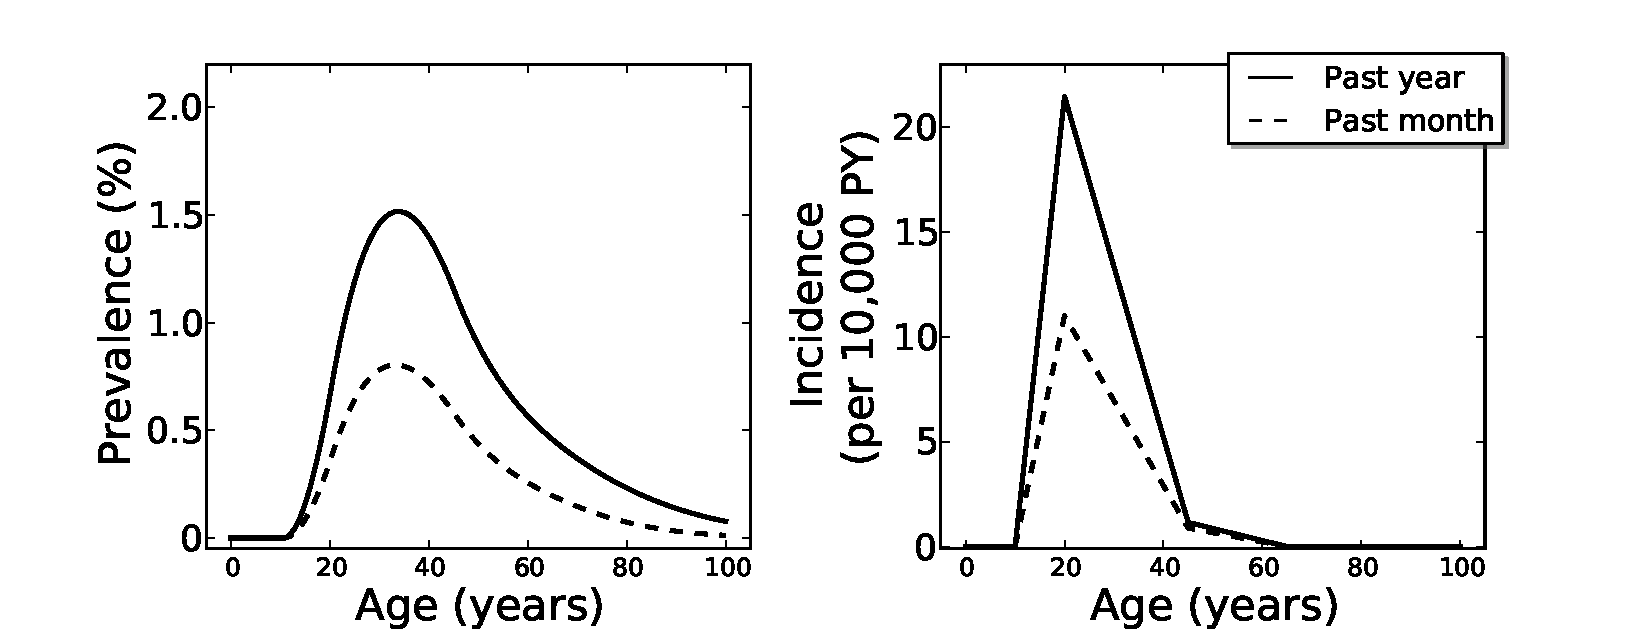
\includegraphics[width=\textwidth]{bipolar-ref-alts.pdf}
\caption{Reference value for the past year/past month prevalence
  covariate has a substantial effect on incidence estimates.  Because
  consistency is enforced at the reference value level, choosing reference
  values is an important modeling decision.}
\label{bipolar-ref-alts}
\end{center}
\end{figure}


Normalization is also important, although it does not affect
consistency.  It is important for stability of numerical algorithms,
and also because the prior on the effect coefficient must be matched
to the scale of the covariate.  Normalizing continuous covariates to
have variance one, for example, means that the prior of
$\beta\sim\Normal(0,1^2)$ is weakly informative.  If a continuous
covariate had variance $0.0001$, the same prior on $\beta$ would be
very informative.

\section{Fixed effects to predict out of sample}

In addition to study-level covariates, like the cross-walks in the
previous section, covariate modeling can be as ``country-level
covariates'' to improve prediction out-of-sample.  Mathematically, the
setting is identical, where a country-level covariate matrix $X'_i$ holds
the value of the covariates, and an effect coefficient parameter
$\beta'$ controls the prediction, multiplying $h$ by
$e^{\beta' X'_i}$.  Conceptually, this deserves a seperate treatment,
  however, because the use and the results are quite different.

A case where the benefit of using fixed effects to predict out of
sample is clear is when modeling an often fatal condition, like cancer
of the pancreas.  Incidence of pancreatic cancer is available from
cancer registries for some regions, but population-level mortality
caused by this condition has been modeled in detail for all
countries.\cite{CODEm_paper}  By using the log of the age-standardized mortality rate as a
covariate in the incidence model, it is possible to borrow strength
from the mortality estimates to inform the incidence estimates.

This approach can also be helpful for covariates that are not as
direct, for example using gross domestic product as an explanatory
covariate for estimating the prevalence of eating disorders, using
estimates of age-standardized Hepatitis C Virus prevalence as an
explanatory covariate for estimating prevalence of cirrhosis, or using
an indicator for violent conflict as an explanatory covariate for
estimating the prevalence of depression and anxiety.



\section{Fixed effects to explain variance}
Fixed effect modeling in the previous sections has focused on
improving predictions of the mean of observed data.  It is also
possible to use fixed effect covariate modeling to explain the
different levels of variation in different sources of data, which is
the topic of this section.

To introduce this idea by way of example, consider the results of the
systematic review for Hepatitis C Virus seroprevalence.  This
literature search excluded studies in subpopulations known to have
systematic bias, such as studies of prevalence in intravenous drug
users, or paid blood donors.  But it did collect measurements from
studies in subpopulations that were \emph{not} known to be
systematically biased, for example studies that used voluntary blood
donors as the sample frame.  This is clearly not the whole population,
but as it is not known to be a biased sample, I would like to include
it if possible.  This is where using a fixed effect to explain
variation is appropriate. In the systematic review, observations corresponding
the voluntary blood donors, as well as other studies of nonrepresentative
subpopulations, such as mothers visiting antenatal clinics, were
associated with a
bias indicator $Z_i = 1$.  Observations from studies of the general
population received bias indicator $Z_i = 0$.  Then I can
introduce fixed effect coeficient analogous to the previous sections,
but modifying the over-dispersion term of the rate model, instead of
the mean.

This has the following
formulation:
\begin{align*}
r_i &\sim \scD\left(\mu_i, \delta_i; n_i\right),\\
\mu_i &= h(a_i)e^{\beta X_i},\\
\delta_i &= e^{\eta + \zeta Z_i}.
\end{align*}

\section{Random effects for spatial variation}
Another important use of covariates is in handling nonsampling
variation that \emph{cannot} be explained. As I have mentioned
repeatedly, the descriptive epidemiological data available is often
very noisy.  It is usually only a small part of this ``noise'' that
can be explained with covariates like those from the preceding
section. And while the additional variation has no simple explanation
in terms of differing diagnostic criteria or the like, there is
structure in the variation. Countries in the North Africa/Middle East
region have rates more similar to each other than to countries in the
North America, High Income region.  And the North America, High Income
region as a whole is more similar to the Europe, Western region than
to the Asia, South region.  Capturing this spatial similarity when it
exists is the goal in my random effects modeling.

I will develop this approach to random effects modeling by beginning
with something very similar to the fixed-effects model.  The random
effects come in part through the use of additional priors, either
modeling the dispersion of the effects as a parameter itself to be
fit from the data, or going further to model the joint distribution of
spatially neighboring effects to have sums equal to zero.  For
notation, let $U_i$ be a vector of random effect covariates.  This
$U_i$ is a \emph{design matrix} analogous to the fixed-effect
covariate vector $X_i$ above, but with zero/one values corresponding
to the place in the spatial hierarchy to which observation $i$ refers.

In the GBD 2010 study, the spatial hierarchy is countries nested in regions
nested in super-regions, but in national or subnational analyses, the
hierarchy will be different. This can be generically formulated using
graph theory, where a directed tree (also known as an
\emph{out-arborescence}) encodes the hierarchical relationship
structure with a root node connected by out-arcs to children on the
first level of the hierarchy, which are each in turn connected by
out-arcs to children on the next level of the hierarchy, and so on.  A
node is called the \emph{parent} of any node it points to in this
tree, and two nodes are called \emph{siblings} if they share the same
parent.


Analogously to the fixed effect model above, the random effects apply
a multiplicative shift to the age-specific rate function:
\begin{align*}
r_i &\sim \scD\left(\mu_i, \delta_i; n_i\right),\\
\mu_i &= h(a_i)e^{\alpha U_i}.
\end{align*}
The first difference between the fixed effects and random effects is
in the priors on the effect coefficients.  Instead of a weakly
informative prior as above, the prior on $\alpha$ is itself part of
the model, parameterized as:
\[
\alpha_j \sim \Normal\left(0, \sigma_{\ell(j)}^2\right),
\]
where $\ell(j)$ is the level in the hierarchy of node $j$, and
$\sigma_\ell$ is also a model parameter. To fit this model with
Bayesian methods, we also need a prior on $\sigma_\ell$ (a
hyper-prior), and because of the sparse and noisy nature of the
available data, this often has to be somewhat informative.  The
truncated normal distribution
\[
\sigma_\ell \sim \Normal_{[.05,5]}\left(.05, .03^2\right),
\]
is often an appropriate choice. It says that between-area variation of
less than 5\% is impossible and more than 15\% is rare.

A second difference between the fixed effects and random effects which
I have sometimes found convenient is
the following: for every node in the spatial hierarchy, I can
constrain the random
effects for all children of that node to sum to zero.  This ``zero-sum
random effect'' has the implication that if there
are no data for some node, then its random effect must be zero.  It
captures the modeling philosophy that random effects represent
unexplained, but true, variation of nodes in the area hierarchy from
the central tendency of their siblings.  Using $H$ to denote the
hierarchy, this constraint can be formalized mathematically as:
\begin{align*}
\sum_{c\in N^+(p)} \alpha_c &= 0, \text{ for all } p \in N;\\
\alpha_c &=0, \text{ for all $c$ such that } \sum_{i} U_i(c) = 0.
\end{align*}

The zero-sum constraint has important implications in consistent
models, because as described above (and shown in
Figure~\ref{bipolar-ref-alts}), consistency is enforced at the
reference level, which for random effects is $U_i = \0$.


\section{Covariates and consistency}
One of the most challenging theoretical issues in covariate modeling
for integrative systems modeling is the interplay between the
predictive covariates and the intercompartmental consistency.  A
simple example of the problem arises in a model of congenital
abnormalities, where there is birth prevalence, but no incidence or
remission, and data on prevalence and cause-specific population
mortality. If covariates are used to shift predictions for the level
of $h_{p}*h_{f}$ as well as the level of $h_{p}$ and the level of $h_{f}$, then
consistency would require that $\beta^{h_{pf}}_i = \beta^{h_p}_i + \beta^{h_f}_i$.

This complication becomes even more pronounced in a model where there
is nonzero incidence and remission.  In the general case, it is not
even clear that nonzero covariate effects exist that respect
consistency.

To circumvent this challenge, I have used a multistage approach to
fitting the model (see Section~\ref{empirical-priors}), and at each
stage of the process, there is a specific level of the hierarchical
model where I have enforced the consistency conditions of the system
dynamics model.  All predictions from this stage apply only to this
node and nodes lower in the hierarchy, and for the lower nodes, the
predictions are not consistent.  However, they are expected to
be close to consistent, a hypothesis that must be investigated
empirically on a case-by-case basis.

How does this work?  Recall the covariate model formulation for
predicting the rate for a given geographic area, sex, and year $(g,s,y)$:
\[
\boldpi_{g,s,y}(a) = h(a)e^{\alpha U_{g,s,y} + \beta X_{g,s,y}}.
\]
For the highest node of the hierarchy (also called the
\emph{reference} node, and corresponding to geographic area/sex/year $(g_r, s_r,
y_r)$), I simply apply a linear shift to each covariate in $X$ and $U$
to have $X_{{g_r},{s_r},{y_r}} = \0$ and $U_{g_r,s_r,y_r} = \0$.  This
simplifies to \[ \boldpi_{g_r,s_r,y_r}(a) = h(a), \] and for any system
of differential equations that $\{h_t(a), t=[T]\}$ are
solutions, the predicted values for the age, sex, year at the root of
the hierarchy are also solutions.

An important direction for future work is to go beyond the multistage
approach.  This will probably require innovation in algorithms,
because fitting multiple consistent models simultaneously is currently
impractical.

\section{Identifiability}
The random effects modeling approach described above must be
implemented with caution.  In a naive implementation, the effects at
the super-region, region, and country level will interact in a way
that leads to ``nonidentifiability''.  While this is not a
theoretical limitation in the Bayesian framework, it has practical
ramifications: the Markov chain Monte Carlo algorithm will not converge well when there
are many random effects that can all do the same job.  To avoid this,
it is important to carefully choose which area random effects to include.

